%・(PC側では)クリックした人間の映像を正面に持ってくることで,正面を見ていれば見たい人を物理的にも見ているという状態を作る

%・(OEB側では)PC側が見ている特定の個人の方向に,PC使用者の顔を映す

%・残りの人間には,PC側と,見ている人間の顔を小さいウインドウに移し,視線情報と通信相手の顔を伝える

%・特定の1人を見ていない状況を区別するため,そのような状況下では全員にPC使用者の顔を小さいウインドウに移す

PC側で提案するシステムを以下に述べる.平面ディスプレイ上に
OmniEyeBallに取り付けた全天球ビデオカメラのパノラマ映像を表示する.
映像上で,参加者の顔をクリックすることで,その参加者が正面に来るように
パノラマ映像を平行移動させる.そのようにして,常に正面を見ていれば
見たい人を見ているという状態を作り出す.

%(ここに,画像をスライドさせる図を乗せる)
\begin{figure}[tbp]
  \centering
  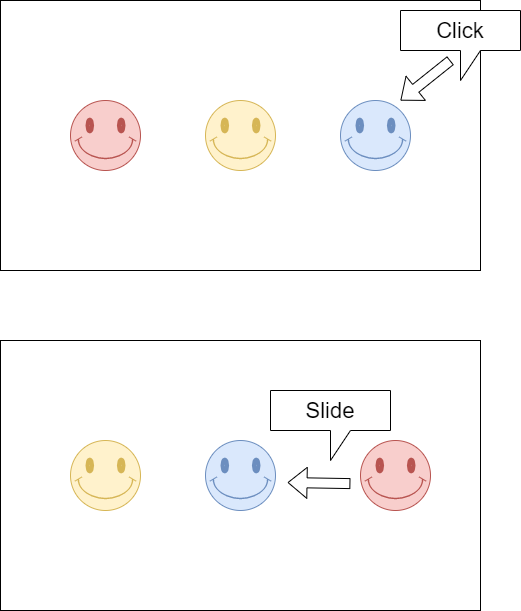
\includegraphics[scale=0.6]{fig/PCsideSlide.png}
  \caption{全天周パノラマ画像のスライド}
\end{figure}

以降は,OmniEyeBall側で提案するシステムを述べる.
PC側で使用する全天周ビデオカメラの映像を
球体ディスプレイ上に表示する.PC側のクリック操作に合わせ
クリックされた人物の方向に顔が向くように映像を回転させる.
こうすることで,PC側で見ている人間とみられた人間が向き合う状態を作る.

\begin{figure}[tbp]
  \centering
  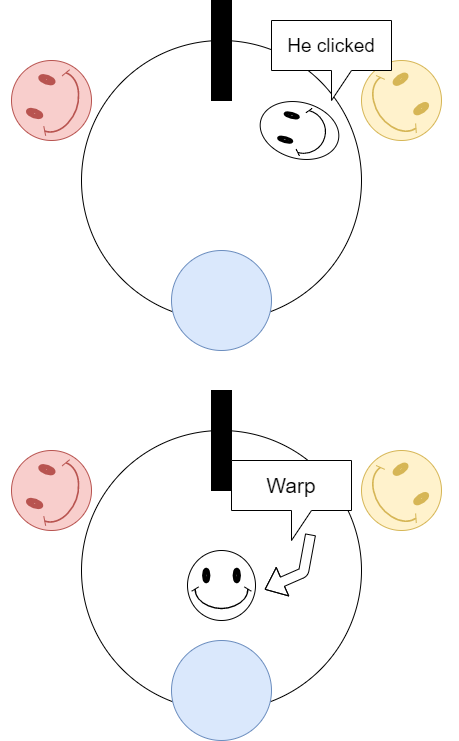
\includegraphics[scale=0.6]{fig/OEBsideSlideimg.png}
  \caption{クリックイベント発生時の全天球ディスプレイ上の表示}\label{OEBGUI1}
\end{figure}

この時,例えば3人が120度の間隔でOmniEyeBallの周りに座っている状況を考えると,
顔を向けられていない2人は,ほとんどPC側の参加者の顔を視認できない.
このような場合,この2人には画面上部に小さなウインドウを表示し,そこに
PC側参加者の顔部分を表示する.顔部分を表示すると,その顔は大抵正面方向を向いており
,自身が見られていると錯覚する恐れがある.それを防ぐため,PC参加者の顔ウインドウ
の隣には,見られている参加者の顔ウインドウを表示させる.

また,このままではPC側の使用者が,特定の個人を見ていない場合
(例えば,全員に対して語りかける場合)を区別できない.このため,
特定の個人を見ていない場合は,全員に対して画面上部に
PC参加者のみの顔ウインドウを表示させる.クリックした人物の方向を向く
仕様では,常に前回のクリックの結果が残り,いずれかの人物の顔方向に
PC参加者の顔が向くことになる.この方向に対して,あえて顔ウインドウ
を顔映像に被せることによって,大きく表示される方の顔映像の視認性を下げ,
自身が見られているという錯覚を防ぐことが狙いである.

\begin{figure}[tbp]
  \centering
  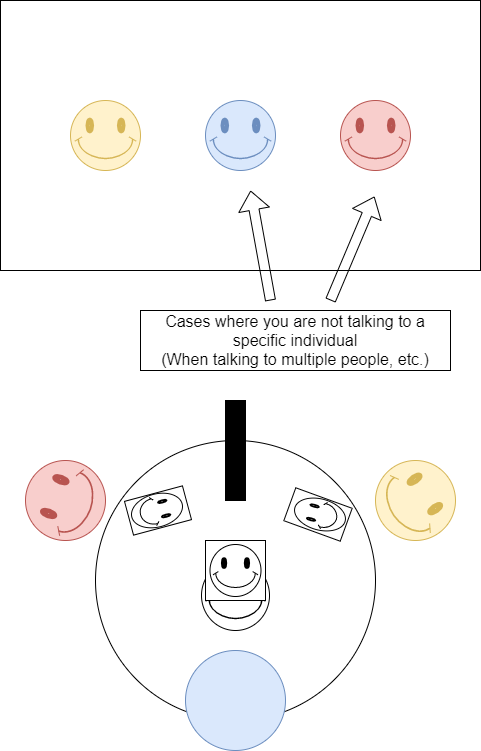
\includegraphics[scale=0.6]{fig/SPcase.png}
  \caption{特定の個人を見ていない場合の表示}\label{OEBGUI2}
\end{figure}

以上で提案したシステムを用いて,従来のビデオ通話アプリケーション
を用いた場合よりもPCの使用者の視線情報がOmniEyeBallの使用者に正確に伝わることが最終的な目標である.